
\documentclass[buriama8_dp.tex]{subfiles}
\begin{document}
\chapter{Coverage path planning}
\label{chap:cpp}

Coverage Path Planning (\textit{CPP}) is \quot{the task of determining a path that passes over all points of an area or volume of interest while avoiding obstacles}{survey13}. The task comes naturally with different robotic applications, where the robot is to complete some task in every point in the environment.

The problem has been studied both practically and theoretically. In literature, the problem of planning an optimal covering route is referred to as the \uvz{lawnmower problem} or the \uvz{milling problem} and has been shown to be NP-hard \cite{lawnmowing}. The methods below either don't give any optimality guarantees, or hide the complexity elsewhere, as solving an integer LP.

\section{Applications}
The first such task that comes to mind is of course cleaning. This sometimes tedious task has been in focus of the robotics community for quite some time, with articles concerning this topic dating back to 1988 \cite{cleaning88}. Other applications studied include painting, de-mining, automated agricultural vehicles and so on \cite[sec.~1]{survey13}.


\section{Approach families}

Several different approaches to the problem appeared over time. A typical application takes place in a 2-dimensional, previously known environment. We will introduce several inspiring methods of 2D coverage, and then present a scheme to generalize them to 3D.

\TODO{define workspace, obstacle}

\subsection{Random strategies}
\label{subsec:random_cpp}
The simplest coverage strategy is a random strategy. The environment is traversed completely randomly, and, hopefully, most of the environment will have been covered at some point in the future. Random strategies are commonly used in vacuum cleaning robots because they do not require any expensive special hardware and are easy to implement. As the robots are autonomous and work when their owner is not at home, optimal performance is not crucial.

Vacuum cleaners following random strategies have been shown to perform relatively well in terms of converging to fully cleaned room in reasonable time~\cite{randomcover}.

In our case, time is a scarce resource and we need to cover the whole area in the least time possible. The great advantage of random planning is the fact that it does not need any prior information about the environment, which is the characteristic we are looking for in our method of choice.

\subsection{Heuristic methods}
\label{subsec:heuritic}
Next in line with simplicity are heuristic strategies. \cite{rt_heuristic_coverage} describes several such strategies. All of them are used in grid map representation.

The simplest strategy is closest-first, which randomly chooses an uncovered field adjacent to the current one; if none such exists, a BFS is performed to find the closest uncovered field and navigates to it.

To improve the results of the aforementioned heuristic, we augmented it by providing it clues on which field to choose. Our heuristic and the rationale behind it is described below in Section~\ref{sec:my_heuristic}.

Another heuristic method used is a modification of the WaveFront method \cite{wavefront} to unknown environments, called Iterated WaveFront. In the WaveFront method, the environment is traversed along cells equidistant to a goal state selected beforehand. This should ensure that all the far areas will have been covered when we get close to the goal, thus making the coverage as efficient as possible. Iterated WaveFront selects the goal state randomly, computing path in the currently known map. When an obstacle is encountered, the plan is recomputed over the updated map.

Heuristic strategies do not provide any optimality guarantees, and can perform very badly in the worst cases. They are however very easy to implement, and can cope with unknown environments well. 

\subsection{Exact cellular decomposition}
\label{subsec:label}
When the environment is known and can be represented, or at least approximated, by polygons or differential functions, exact cellular decomposition approaches can be used. This family of approaches performs a decomposition of the workspace with obstacles into distinct cells. The cells are then traversed and each is covered by a trivial zig-zag pattern, sometimes called the \textit{boustrophedon pattern}, an example of which can be seen in Figure~\ref{fig:zig_pattern}. The traversal order is where the complexity is hidden in this technique.

\begin{figure}[ht]
  \centering
  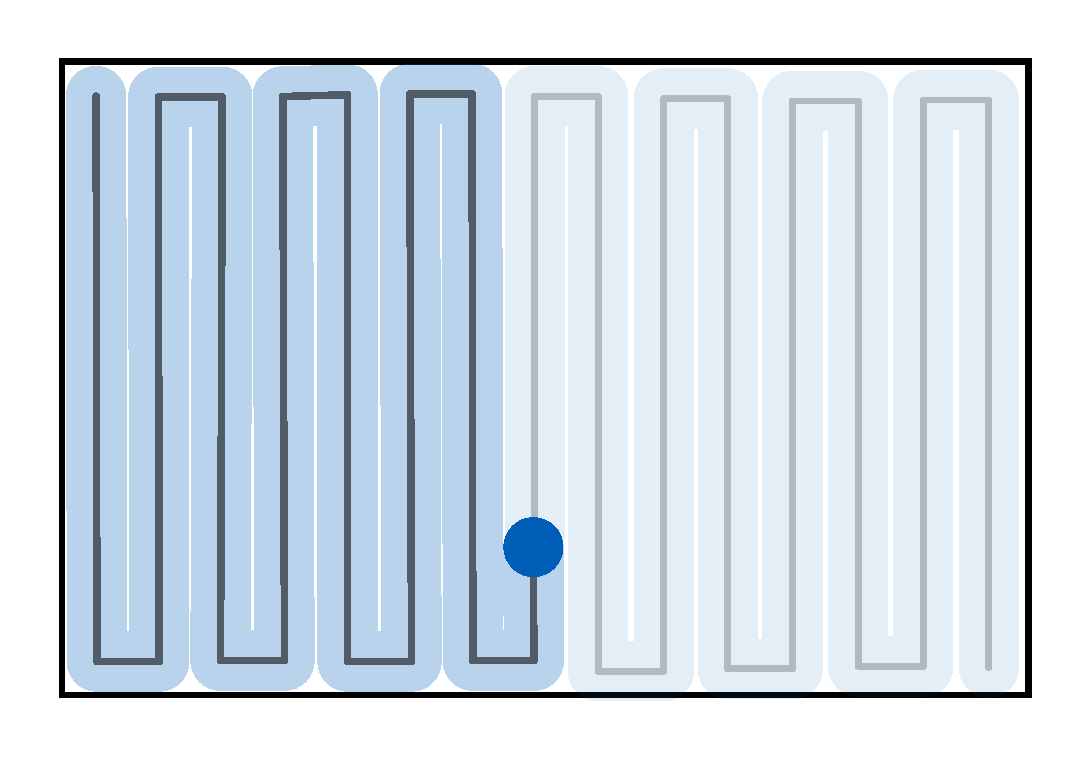
\includegraphics[width=6cm]{figures/zigzag.pdf}
  \caption[Boustrophedon pattern]{Example of the boustrophedon or zig-zag pattern. The environment is sequentially covered by the advancing sweeps}
  \label{fig:zig_pattern}
\end{figure}

The two commonly used decomposition techniques are trapezoid decomposition and boustrophedon decomposition. Trapezoid decomposition is usually used to index point location in planar decomposition. Here, only the exterior of obstacle polygons is decomposed. Then an adjacency graph of the cells is created and a path through the graph is computed, visiting every cell (vertex) at least once. As the path is followed, each cell is covered by the zig-zag pattern, and then the robot moves to the next cell.

The trapezoidal decomposition typically generates many adjacent cells that could be merged and still traversed trivially, but more efficiently, because less border areas will need to be handled. The boustrophedon decomposition is similar to the trapezoidal, only certain cells are merged together, eliminating suboptimal coverage of their boundaries. Examples of the two decompositions are presented in Figure~\ref{fig:decomps}.

\begin{figure}[ht]
  \begin{subfigure}[t]{0.4\textwidth}
    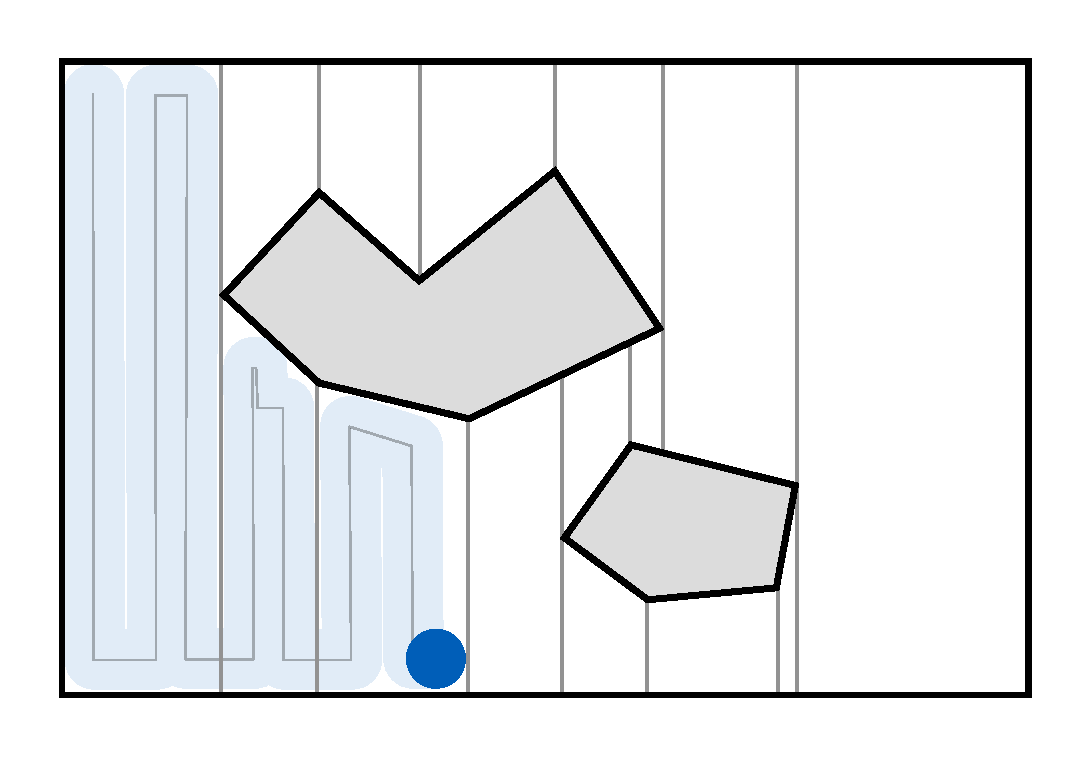
\includegraphics[width=\textwidth]{decomp_trapez.pdf}
    \caption{}
    \label{fig:decomp_trapez}
  \end{subfigure}
  \begin{subfigure}[t]{0.4\textwidth}
    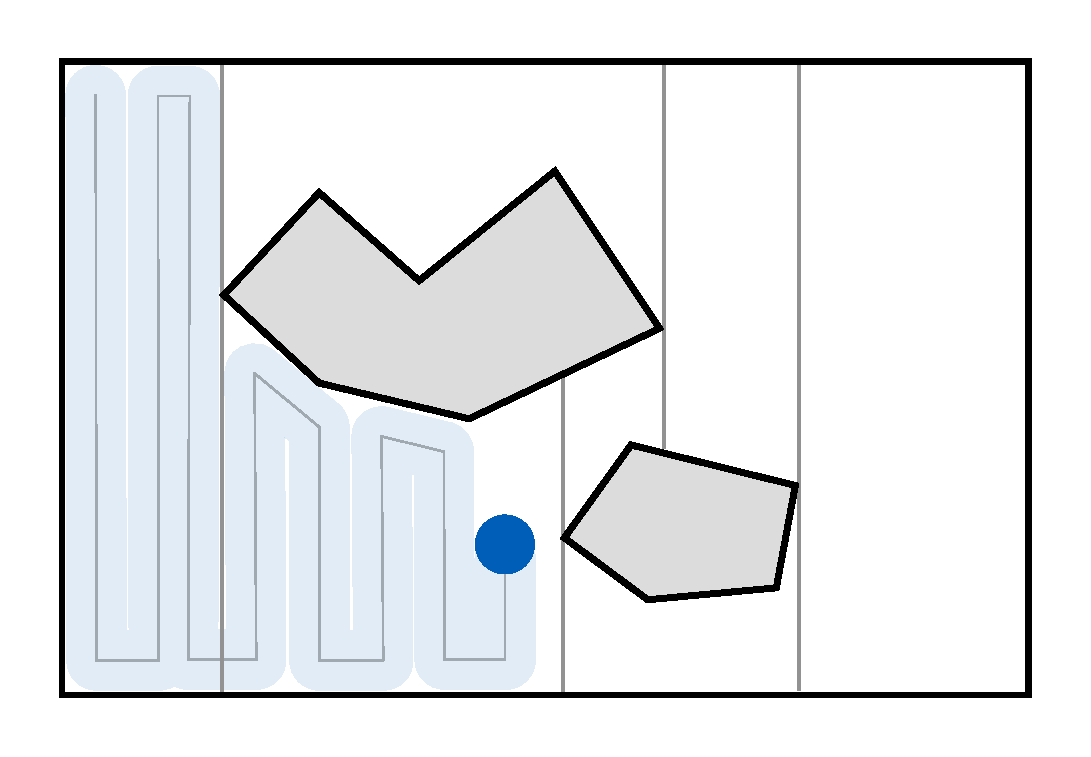
\includegraphics[width=\textwidth]{decomp_boustrop.pdf}
    \caption{}
    \label{fig:decomp_boustrop}
  \end{subfigure}

  \caption[Trapezoid and boustrophedon decompositions]{Example environment decomposed by trapezoid (\subref{fig:decomp_trapez}) and boustrophedon (\subref{fig:decomp_boustrop}) decomposition, with an example of covering path}
  \label{fig:decomps}
\end{figure}

This class of methods is best for perfectly known environments, which is not our case. We mention it to show how exact solutions in known environments can work.

\TODO{CCr?}

\subsection{Grid neural network}
\label{subsec:nncpp}
When the environment is represented in a grid, a neural network-like structure can be used to generate a covering path \cite{neural}. Each cell is represented by a neuron, connected to its 8-neighborhood. The dynamics of the network is described by the short term memory shunting equation for activity \(x_j\) of neuron \m j derived from the physical model of neuron \cite[sec.~III]{neural}
 
\begin{equation}
  \frac{\diff x_j}{\diff t} = -Ax_i + (B-x_i) \left( [I_i]^+ + \sum_{j \in N_i} w_{ij}[x_j]^+ \right) - (D+x_i)[I]^-
\label{eqn:shunting}
\end{equation}

\noindent where \([x]^+=\max\{x,0\}\), \([x]^-=\max\{-x,0\}\); \m A, \m B and \m D are model parameters, \(N_i\) is the set of neighboring neurons to neuron \m i and \(I_i\) is the external input of neuron \m i. According to the authors of the algorithm, the network driven by this model is a stable system proven to be bounded in \([-D,B]\) \cite{grossbergmodel}.

The external input represents the state of exploration of the environment. In unknown fields, it is set to a large constant \m E and thus creates high activity in the area. In known fields, it is set to 0, to allow external activities to propagate. In obstacles, it is set to \(-E\), to locally repulse the robot. From Equation~\ref{eqn:shunting} we can see that positive activity propagates through the network, globally attracting the robot to more active areas, while negative activity is restricted to only the neuron with negative external input.

The robot moves through the network, following the highest activity while taking minimization of the number of turns into consideration. As it moves, it marks the visited fields and adjusts the network input. The network is numerically simulated, advancing time at each robot step.

The great advantage of this method is in its ability to represent and cope with dynamic obstacles. When an obstacle appears, the robot can only update the external input of the respective neuron and the map and trajectory will adjust. This allows us to run the algorithm in completely unknown environment. The algorithm does not give any optimality guarantees, and since its authors' experiments included a ranged sensor, while we only work with contact sensing, the algorithm will be making much less informed decisions in our case.

\section{Compact space heuristic}
\label{sec:my_heuristic}

The closest-first heuristic is the obvious trivial heuristic for the CPP. It only needs to make a reasonable guess on where to go next. 

We designed a simple rule the robot follows. We define the heuristic function \(f\) on cell \m x as 
\[
f(x)= \left\{
    \begin{array}{l}
      |\{i \in N_x | i \textit{ has been explored}\}| + |\{j \in N_x | j \textit{ is a known obstacle}\}| \\
      \hphantom{0} \quad \textrm{ if }x\textrm{ is unvisited} \\
      0 \quad \textrm{ otherwise.}
    \end{array}
    \right.
\]
The robot in cell \(c\) goes to the unvisited cell
\[n = \argmax_{j \in N_c} f(j).\]

In case of a tie between candidates \(\textit{PN}_c\), the robot breaks it by looking at their neighboring cells and choosing candidate
\[
n = \argmax_{j \in \textit{PN}_c} \sum_{k \in N_j} f(k).
\]
If a tie occurs here as well, a candidate is chosen randomly.

If all the neighboring cells have been visited, the robot goes to the nearest unvisited cell.

This heuristic makes sense from multiple points of view. For one, it encodes the common-sense ideas about how to explore an unknown area. We would like to keep the already explored space as compact as possible, to eliminate future need to come back to inspect a few unexplored fields left behind, thus maximizing the number of already visited neighbors of the next cell. The second term encodes the idea that cells next to an obstacle have a higher probability of being obstacles as well, and it is benefitial to explore them sooner to get this knowledge as early as possible and to be able to exploit it.

The heuristic is also closely connected to the well-known heuristic for the knight's tour (or any other Hamiltonian path) problem. We would like to get a Hamiltonian path, as it would minimize revisited cells and thus path length. The original Warnsdorff's heuristic tells us to \uvz{select the move which connects with the fewest number of further moves}. Pohl's heuristic \cite{knight_heuristic}, based on Warnsdorff's, adds a tie-breaking rule, applying the idea recursively: choose the field whose neighboring fields have the fewest ways to continue. Our heuristic follows this rule exactly: maximizing the number of already explored neighbors is equivalent to minimizing the number of possible next moves.

\TODO{handling edge cells}


\section{Generalization to 3D}

The exact methods presented rely on some of the properties of 2-dimensional space, such as that there is only \uvz{above} and \uvz{below} an obstacle, but there is no \uvz{behind}. This makes their direct generalization to 3D impossible. Most effort in 3D coverage has been put into covering 2D surfaces in 3D space, such as car parts (that need to be covered in paint) or more complex terrain on crop fields (that need to be covered by harvesting machines). We however actually need to cover all the cells in a 3D environment.

In our case, the exploration also needs to take into account the kinematic constraints on the arm pose, as we must not allow any part of the arm except the contact sensor to enter unknown areas to prevent possible hardware damage.

Any planar covering algorithm can be extended to 3D by being applied sequentially to consecutive planes. The idea has been described in \cite{gen3d}, albeit in the context of covering the ocean floor.

In a continuous case, we divide the workspace along one dimension into a collection of planes spaced in intervals corresponding to the robot's sensing diameter. This way, when the robot completely covers two consecutive planes, the space in between them will have been covered as well.

When we represent the environment in a grid, we simply choose to use one dimension of the grid, and then cover each layer of the dimension with a planar grid algorithm.

\section{Method comparison}

Of the methods presented above, the ones applicable to our problem are the neural network approach and the heuristic approach. The exact methods need to know the environment completely, to make sure it is traversed optimally.

\TODO{Why not iterative exact?}

The heuristic approaches and the NN approach share the common scheme of selecting a path locally, and moving to the closest unknown cell if no such path can be found. 

In the heuristic methods, the criterion upon which the local decision is based is strictly local and the global view is taken into account only when the local fails.

In the NN, the global signal propagates through the whole environment and thus the state of the whole map impacts the local decision. No hand-crafted global strategies are neccessary. In the end, however, the strategy still boils down to local exploration followed by moving to the globally closest unexplored place when there is nowhere else to go.

The choice of the nearest unclean place is implicit  in the case of neural networks, as the dynamics of the network drive the propagation of activity from unvisited areas such that the signal gets weaker with every step, resulting in the robot going to the closest source of activity via the shortest path when traversing already visited fields.

The heuristic methods have the chioce of the place whence to continue the exploration hand-designed in them. This way, we can design the choice to suit our needs the best.  I our case, this is an advantage, as, because we are working with a robotic arm in three dimensions, we can get to all the fields in our environment directly, without being constrained by planning in a grid with obstacles.




\end{document}

%%% Local Variables:
%%% mode: latex
%%% TeX-master: "buriama8_dp"
%%% End:
%  LocalWords:  CPP
